\documentclass[tikz,border=5pt]{standalone}
\usepackage{tikz}
\usetikzlibrary{arrows.meta}
\definecolor{nebula}{HTML}{6366F1}
\definecolor{spark}{HTML}{14B8A6}
\definecolor{ink}{HTML}{334155}
\begin{document}
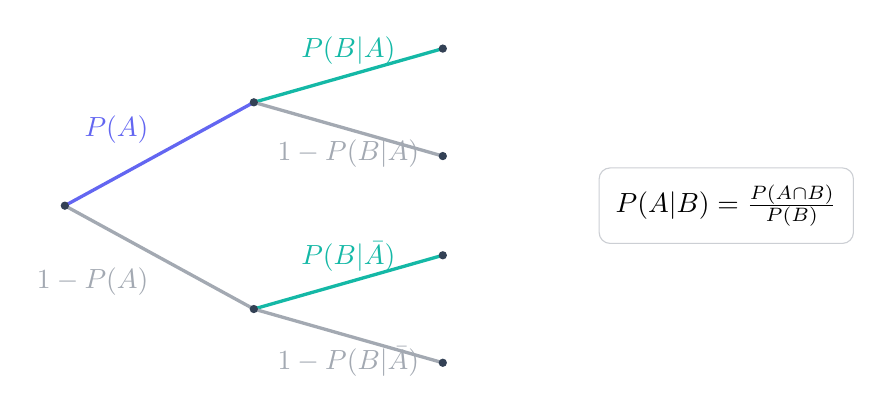
\begin{tikzpicture}[font=\sffamily,>=Latex,x=2.4cm,y=1.05cm]
  \coordinate (o) at (0,0); \coordinate (a) at (1,1.25); \coordinate (na) at (1,-1.25);
  \coordinate (ab) at (2,1.9); \coordinate (anb) at (2,.6);
  \coordinate (nab) at (2,-.6); \coordinate (nanb) at (2,-1.9);
  \draw[very thick,nebula] (o)--(a) node[midway,above left] {$P(A)$};
  \draw[very thick,ink!45] (o)--(na) node[midway,below left] {$1-P(A)$};
  \draw[very thick,spark] (a)--(ab) node[midway,above] {$P(B|A)$};
  \draw[very thick,ink!45] (a)--(anb) node[midway,below] {$1-P(B|A)$};
  \draw[very thick,spark] (na)--(nab) node[midway,above] {$P(B|\bar A)$};
  \draw[very thick,ink!45] (na)--(nanb) node[midway,below] {$1-P(B|\bar A)$};
  \foreach \p in {o,a,na,ab,anb,nab,nanb}{\fill[ink] (\p) circle (1.5pt);}
  \node[draw=ink!25,rounded corners=4pt,fill=white,inner sep=6pt] at (3.5,0)
    {$P(A|B)=\frac{P(A\cap B)}{P(B)}$};
\end{tikzpicture}
\end{document}
